% Deep Learning

\textframe{Time to go Deeper}

\begin{frame}
  \begin{quote}
    What if the meaning of life is to spend your time thinking about the meaning of life?
  \end{quote}
\end{frame}

\begin{frame}
  \centering
  {
    \Huge
    \color{orange}
    Deep Learning
    \vspace{0.5cm}
  }

  {
  \Large
  \pause The why\pause, the what\pause{} and the ugly.
  }
\end{frame}

\begin{slide}{Deep Learning}
  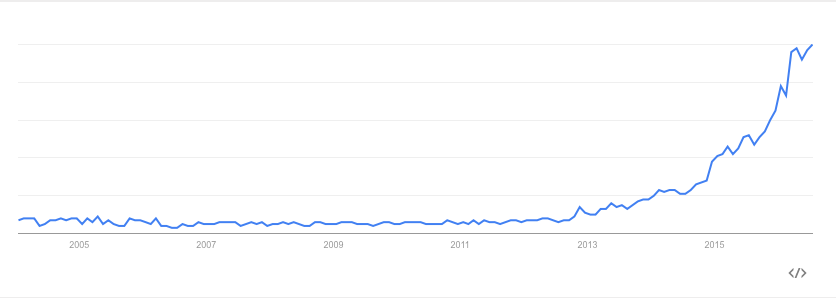
\includegraphics[scale=0.3]{dl-trend}
\end{slide}

\begin{slide}{Deep Learning}
  \frameheader{Basic Definition}

  \begin{itemize}
    \pitem Let $\mathcal{L}$ denote the number of hidden layers in a neural network
    \pitem Then we call neural network \emph{deep}, if
    \begin{enumerate}
      \pitem It is trained at more than 10,000m below sea level, or
      \pitem $\mathcal{L} > 1$
    \end{enumerate}
    \pitem To really understand why many layers are a good idea, we must understand why few layers might be a bad idea
  \end{itemize}
\end{slide}

\begin{slide}{Universal Approximation Theorem}
  \begin{itemize}
    \pitem Theoretically, a single layer is just enough
    \pitem However, we would need exponentially many units for discrete functions
    \pitem And infinitely many for continuous functions
    \pitem Just use an infinitely sized hash table

    % Say this, don't put it on the slides!
    % \pitem Unfortunately, infinity does not scale well
    % \pitem Even with Hadoop
    % \pitem Example:
    % \begin{itemize}
    %   \pitem If we have five boolean inputs, each can take on two states
    %   \pitem In total, that gives $2^5 = 32$ possible input configurations
    %   \pitem Just make the hidden layer a lookup table with 32 entries
    %   \pitem Each fires for one configuration and yields the corresponding output
    %   \pitem Profit
    % \end{itemize}
  \end{itemize}
\end{slide}

\begin{slide}{The Curse of Dimensionality}
  \begin{itemize}
    \item<2-> The number of possible outputs scales exponentially with the dimensionality of our dataset
    \item<3-> Assume our features have 10 possible values
  \end{itemize}
  \only<-3>{\vspace{2cm}}
  \only<4-9>{
  \vspace{1cm}
  \begin{tikzpicture}
    \foreach \i in {0, ..., 4} {
      \draw ({\i*0.4}, 0) rectangle ++(0.4, 0.4);
      \draw ({-(\i + 1)*0.4}, 0) rectangle ++(0.4, 0.4);
    }

    % During training we are filling out these spaces
    % 50% trained!
    \only<5-9>{\draw [fill=red] (0, 0) rectangle ++(0.4, 0.4);}
    \only<6-9>{\draw [fill=cyan] (0.8, 0) rectangle ++(0.4, 0.4);}
    \only<7-9>{\draw [fill=orange] (-1.2, 0) rectangle ++(0.4, 0.4);}
    \only<8-9>{\draw [fill=purple] (1.2, 0) rectangle ++(0.4, 0.4);}
    \only<9-9>{\draw [fill=Green] (-2, 0) rectangle ++(0.4, 0.4);}

    \draw (0, -0.5) node {$1 \text{ feature } = 10 \text{ outputs }$};
  \end{tikzpicture}
  }
  \only<10-15>{
  \vspace{0.5cm}
  \begin{tikzpicture}
    \foreach \x in {0, ..., 9} {
      \foreach \y in {0, ..., 9} {
        \draw ({\x*0.4}, {\y*0.4}) rectangle ++(0.4, 0.4);
      }
    }

    % During training we are filling out these spaces
    % 50% trained!
    \only<11-15>{\draw [fill=red] (0, 0) rectangle ++(0.4, 0.4);}
    \only<12-15>{\draw [fill=cyan] (2.4, 2.4) rectangle ++(0.4, 0.4);}
    \only<13-15>{\draw [fill=orange] (3.2, 1.6) rectangle ++(0.4, 0.4);}
    \only<14-15>{\draw [fill=purple] (1.2, 3.6) rectangle ++(0.4, 0.4);}
    \only<15-15>{\draw [fill=Green] (1.6, 1.2) rectangle ++(0.4, 0.4);}

    \draw (2, -0.5) node {$2 \text{ features } = 100 \text{ outputs }$};
  \end{tikzpicture}
  }
  \only<16->{
  \vspace{0.2cm}
  \begin{tikzpicture}
    % \foreach \x in {0, ..., 9} {
    %   \foreach \y in {0,...,  9} {
    %     \foreach \z in {0,...,  9} {
    \foreach \x in {0, 9} {
      \foreach \y in {0, 9} {
        \foreach \z in {0,  9} {
        \begin{scope}[canvas is yx plane at z={\z*0.4}]
          \draw [help lines] ({\x*0.4}, {\y*0.4}) rectangle ++(0.4, 0.4);
        \end{scope}
        \begin{scope}[canvas is zx plane at y={\y*0.4}]
          \draw [help lines] ({\x*0.4}, {\z*0.4}) rectangle ++(0.4, 0.4);
        \end{scope}
        \begin{scope}[canvas is yz plane at x={\x*0.4}]
          \draw [help lines] ({\y*0.4}, {\z*0.4}) rectangle ++(0.4, 0.4);
        \end{scope}
        \ifnum\x=9
          \begin{scope}[canvas is yz plane at x=4]
            \draw [help lines] ({\y*0.4}, {\z*0.4}) rectangle ++(0.4, 0.4);
          \end{scope}
          \begin{scope}[canvas is xy plane at z=0]
            \draw [help lines] ({\y*0.4}, {\z*0.4}) rectangle ++(0.4, 0.4);
          \end{scope}
        \fi
        }
      }
    }

    \draw (5, 1.5, 0)
          node [rotate=90] {$3 \text{ features } = 100 \text{ outputs }$};
  \end{tikzpicture}
  }
\end{slide}

\begin{slide}{The Curse of Dimensionality}
  \begin{itemize}
    \item Why is this a problem?
    \pitem To predict an output, we must have seen at least one example  % to say if a picture contains a dog, we must know what a dog looks like
    \pitem In high dimensions, an algorithm cannot possibly be trained on all possible output\pause, unless
  \end{itemize}
  \vspace{0.5cm}
  \pause
  {\LARGE We make assumptions about our data}
\end{slide}

\begin{slide}{The Curse of Dimensionality}
  \begin{itemize}
    \item<1-> Assumptions either
    \begin{itemize}
      % When mapping images to 10-letter captions, not all 10-letter strings will be valid outputs. So we have reduced the output space
      \item<2-> Explicitly reduce the output space, or
      \item<3-> Create dependencies between outputs
    \end{itemize}
    \item<4-> \emph{Local constancy} assumption (prior) $$f^\star(\mathbf{x})
     \approx f^\star(\mathbf{x} + \varepsilon)$$
     % The pixels might not quite correspond to this race of dog, but it's still similar to it, so we call it a dog (unless we have better examples)
    \item<7-> Don't need as much data any more!
  \end{itemize}
  \onslide<5->{
  \vspace{0.5cm}
  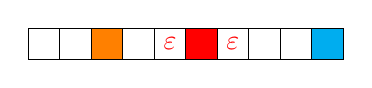
\begin{tikzpicture}
    \foreach \i in {0, ..., 4} {
      \draw ({\i*0.4}, 0) rectangle ++(0.4, 0.4);
      \draw ({-(\i + 1)*0.4}, 0) rectangle ++(0.4, 0.4);
    }

    % During training we are filling out these spaces
    % 50% trained!
    \draw [fill=red] (0, 0) rectangle ++(0.4, 0.4);
    \draw [fill=cyan] (1.6, 0) rectangle ++(0.4, 0.4);
    \draw [fill=orange] (-1.2, 0) rectangle ++(0.4, 0.4);

    % \only<8-9>{\draw [fill=purple] (1.2, 0) rectangle ++(0.4, 0.4);}
    % \only<9-9>{\draw [fill=Green] (-2, 0) rectangle ++(0.4, 0.4);}

    % Dependencies
    \only<6->{
      \draw (0.4, 0) rectangle ++(0.4, 0.4) node [red, midway] {$\varepsilon$};
      \draw (-0.4, 0) rectangle ++(0.4, 0.4) node [red, midway] {$\varepsilon$};
    }
  \end{tikzpicture}
  }
\end{slide}

\begin{slide}{The Curse of Dimensionality}
  {\Large
    Deep Learning assumes that data is structured\\

    \onslide<2->{
      \vspace{0.5cm}
      {\Huge  hierarchically}
    }
  }
  \vspace{1cm}

  \onslide<3-> {
    \footnotesize
    Note:\\
    According to the \emph{No Free Lunch Theorem} it is just as bad as flipping a coin.
  }
\end{slide}

% Convolutional Neural Networks

\begin{slide}{Convolutional Neural Networks}
  \begin{itemize}
    \item<1-> Convolutional Neural Networks (CNNs; ConvNets) are used in image recognition
    \item<2-> They assume their input are images
  \end{itemize}
  \vspace{0.2cm}
  \only<1>{\vspace{3cm}}
    \only<2>{
    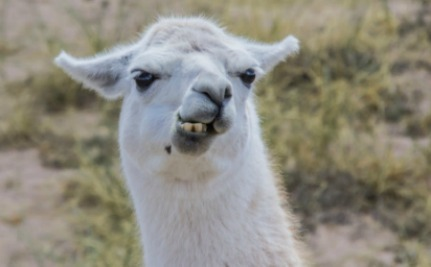
\includegraphics[scale=0.3]{llama}
    }
  \only<3>{
  \begin{tikzpicture}
    % Pixels
      \foreach \x in {0, 0.25, ..., 3.75} {
        \foreach \y in {0, 0.25, ..., 3.75} {
          \randomcolor
          \fill [randomcolor] (\x, \y) rectangle ++(0.25, 0.25);
        }
      }
  \end{tikzpicture}
  }
  \only<4>{
  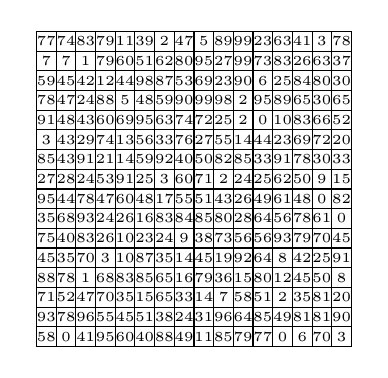
\begin{tikzpicture}
    % Pixels
      \foreach \x in {0, 0.25, ..., 3.75} {
        \foreach \y in {0, 0.25, ..., 3.75} {
          \draw (\x, \y) rectangle ++(0.25, 0.25) node [midway] {\tiny\pdfuniformdeviate 100};
        }
      }
  \end{tikzpicture}
  }
  \only<5->{
  \begin{tikzpicture}
    % R layer (feature map)
    \onslide<8->{
    \yzplane{0}{
      \fill [ProcessBlue] (0, 0) rectangle ++(4, 4);
    }
    % \xyplane{0}{
    %   \fill [ProcessBlue] (0, 0) rectangle ++(0.3, 4);
    % }
    % \xyplane{4}{
    %   \fill [ProcessBlue] (0, 0) rectangle ++(0.3, 4);
    % }
    % \xzplane{0}{
    %   \fill [ProcessBlue] (0, 0) rectangle ++(0.3, 4);
    % }
    % \xzplane{4}{
    %   \fill [ProcessBlue] (0, 0) rectangle ++(0.3, 4);
    % }
    }

    % G layer (feature map)
    \onslide<7->{
    \yzplane{0.6}{
      \fill [Green] (0, 0) rectangle ++(4, 4);
    }
    % \yzplane{0.9}{
    %   \fill [Green] (0, 0) rectangle ++(4, 4);
    % }
    % \xyplane{0}{
    %   \fill [Green] (0.6, 0) rectangle ++(0.3, 4);
    % }
    % \xyplane{4}{
    %   \fill [Green] (0.6, 0) rectangle ++(0.3, 4);
    % }
    % \xzplane{0}{
    %   \fill [Green] (0.6, 0) rectangle ++(0.3, 4);
    % }
    % \xzplane{4}{
    %   \fill [Green] (0.6, 0) rectangle ++(0.3, 4);
    % }
    }

    % B layer (feature map)
    \onslide<6->{
    \yzplane{1.2}{
      \fill [Red] (0, 0) rectangle ++(4, 4);
    }
    % \yzplane{1.5}{
    %   \fill [Red] (0, 0) rectangle ++(4, 4);
    % }
    % \xyplane{0}{
    %   \fill [Red] (1.2, 0) rectangle ++(0.3, 4);
    % }
    % \xyplane{4}{
    %   \fill [Red] (1.2, 0) rectangle ++(0.3, 4);
    % }
    % \xzplane{0}{
    %   \fill [Red] (1.2, 0) rectangle ++(0.3, 4);
    % }
    % \xzplane{4}{
    %   \fill [Red] (1.2, 0) rectangle ++(0.3, 4);
    % }
    }

    % Pixels
    \yzplane{1.8}{
      \foreach \y in {0, 0.25, ..., 3.75} {
        \foreach \z in {0, 0.25, ..., 3.75} {
          \randomcolor
          \fill [randomcolor] (\y, \z) rectangle ++(0.25, 0.25);
        }
      }
    }
  \end{tikzpicture}
  }
\end{slide}

\begin{slide}{Convolutional Neural Network}
  \begin{itemize}
    \item<1-> We want to classify images into one of $k$ classes
    \item<2-> The model should learn to extract features
    \item<3-> We expect it to exploit the hierarchical nature of the data
    \begin{enumerate}
      \item<4-> Lines and edges
      \item<4-> Corners and contours
      \item<4-> Abstract components (e.g. noses, ears, feet)
      \item<4-> Entire objects (e.g. faces, spaceship)
    \end{enumerate}
    \item<5-> First idea: just feed the pixels into a neural network
  \end{itemize}
\end{slide}

\begin{slide}{Convolutional Neural Network}
  $$
  \begin{sbmatrix}{R}
    116 & 80 \\
    170 & 194 \\
  \end{sbmatrix}
  \hspace{0.5cm}
  \begin{sbmatrix}{G}
    82 & 78 \\
    5 & 236 \\
  \end{sbmatrix}
  \hspace{0.5cm}
  \begin{sbmatrix}{B}
    76 & 139 \\
    245 & 236 \\
  \end{sbmatrix}
  $$
  \pause
  \texttt{concatenate(}$R$\texttt{.flatten, }$G$\texttt{.flatten, }$B$\texttt{.flatten}\texttt{)}
\end{slide}

\begin{slide}{Convolutional Neural Network}
  $$
  \begin{sbmatrix}{R}
    116 & 80 \\
    170 & 194 \\
  \end{sbmatrix}
  \hspace{0.5cm}
  \begin{sbmatrix}{G}
    82 & 78 \\
    5 & 236 \\
  \end{sbmatrix}
  \hspace{0.5cm}
  \begin{sbmatrix}{B}
    76 & 139 \\
    245 & 236 \\
  \end{sbmatrix}
  $$
  \begin{align*}
    R\mathtt{.flatten} &= \begin{bmatrix}116 & 80 & 170 & 194\end{bmatrix}
  \end{align*}
\end{slide}

\begin{slide}{Convolutional Neural Network}
  $$
  \begin{sbmatrix}{R}
    116 & 80 \\
    170 & 194 \\
  \end{sbmatrix}
  \hspace{0.5cm}
  \begin{sbmatrix}{G}
    82 & 78 \\
    5 & 236 \\
  \end{sbmatrix}
  \hspace{0.5cm}
  \begin{sbmatrix}{B}
    76 & 139 \\
    245 & 236 \\
  \end{sbmatrix}
  $$
  \begin{align*}
    R\mathtt{.flatten} &= \begin{bmatrix}116 & 80 & 170 & 194\end{bmatrix}\\
    G\mathtt{.flatten} &= \begin{bmatrix}82 & 78 & 5 & 236\end{bmatrix}
  \end{align*}
\end{slide}

\begin{slide}{Convolutional Neural Network}
  $$
  \begin{sbmatrix}{R}
    116 & 80 \\
    170 & 194 \\
  \end{sbmatrix}
  \hspace{0.5cm}
  \begin{sbmatrix}{G}
    82 & 78 \\
    5 & 236 \\
  \end{sbmatrix}
  \hspace{0.5cm}
  \begin{sbmatrix}{B}
    76 & 139 \\
    245 & 236 \\
  \end{sbmatrix}
  $$
  \begin{align*}
    R\mathtt{.flatten} &= \begin{bmatrix}116 & 80 & 170 & 194\end{bmatrix}\\
    G\mathtt{.flatten} &= \begin{bmatrix}82 & 78 & 5 & 236\end{bmatrix}\\
    B\mathtt{.flatten} &= \begin{bmatrix}76 & 139 & 245 & 236\end{bmatrix}
  \end{align*}
\end{slide}

\begin{slide}{Convolutional Neural Network}
  $$
  \begin{sbmatrix}{R}
    116 & 80 \\
    170 & 194 \\
  \end{sbmatrix}
  \hspace{0.5cm}
  \begin{sbmatrix}{G}
    82 & 78 \\
    5 & 236 \\
  \end{sbmatrix}
  \hspace{0.5cm}
  \begin{sbmatrix}{B}
    76 & 139 \\
    245 & 236 \\
  \end{sbmatrix}
  $$

  \begin{align*}
    R\mathtt{.flatten} &= \begin{bmatrix}116 & 80 & 170 & 194\end{bmatrix}\\
    G\mathtt{.flatten} &= \begin{bmatrix}82 & 78 & 5 & 236\end{bmatrix}\\
    B\mathtt{.flatten} &= \begin{bmatrix}76 & 139 & 245 & 236\end{bmatrix}
  \end{align*}

  $$\mathbf{x} = \begin{bmatrix}116,  80, 170, 194,  82,  78,   5, 236,  76, 139, 245, 236\end{bmatrix}$$
\end{slide}

\begin{slide}{Convolutional Neural Networks}
  \begin{itemize}
    \item Why is this a bad idea?
    \begin{enumerate}
      \pitem Fully connected NNs scale badly for images
      \begin{itemize}
        \pitem $200 \times 200 \times 3 = 120,000$ features
        \pitem With 100 hidden units: $100 \times 120,000 = 12,000,000$
        \pitem With 5 layers: $12,000,000 \times 5 = 60,000,000$ weights
        \pitem $1000 \times 1000 \rightarrow 1,500,000,000$ weights
      \end{itemize}
      \pitem It assumes every pixel has entirely new information
    \end{enumerate}
  \end{itemize}
\end{slide}

\begin{slide}{Convolutional Neural Networks}
  \only<1>{
    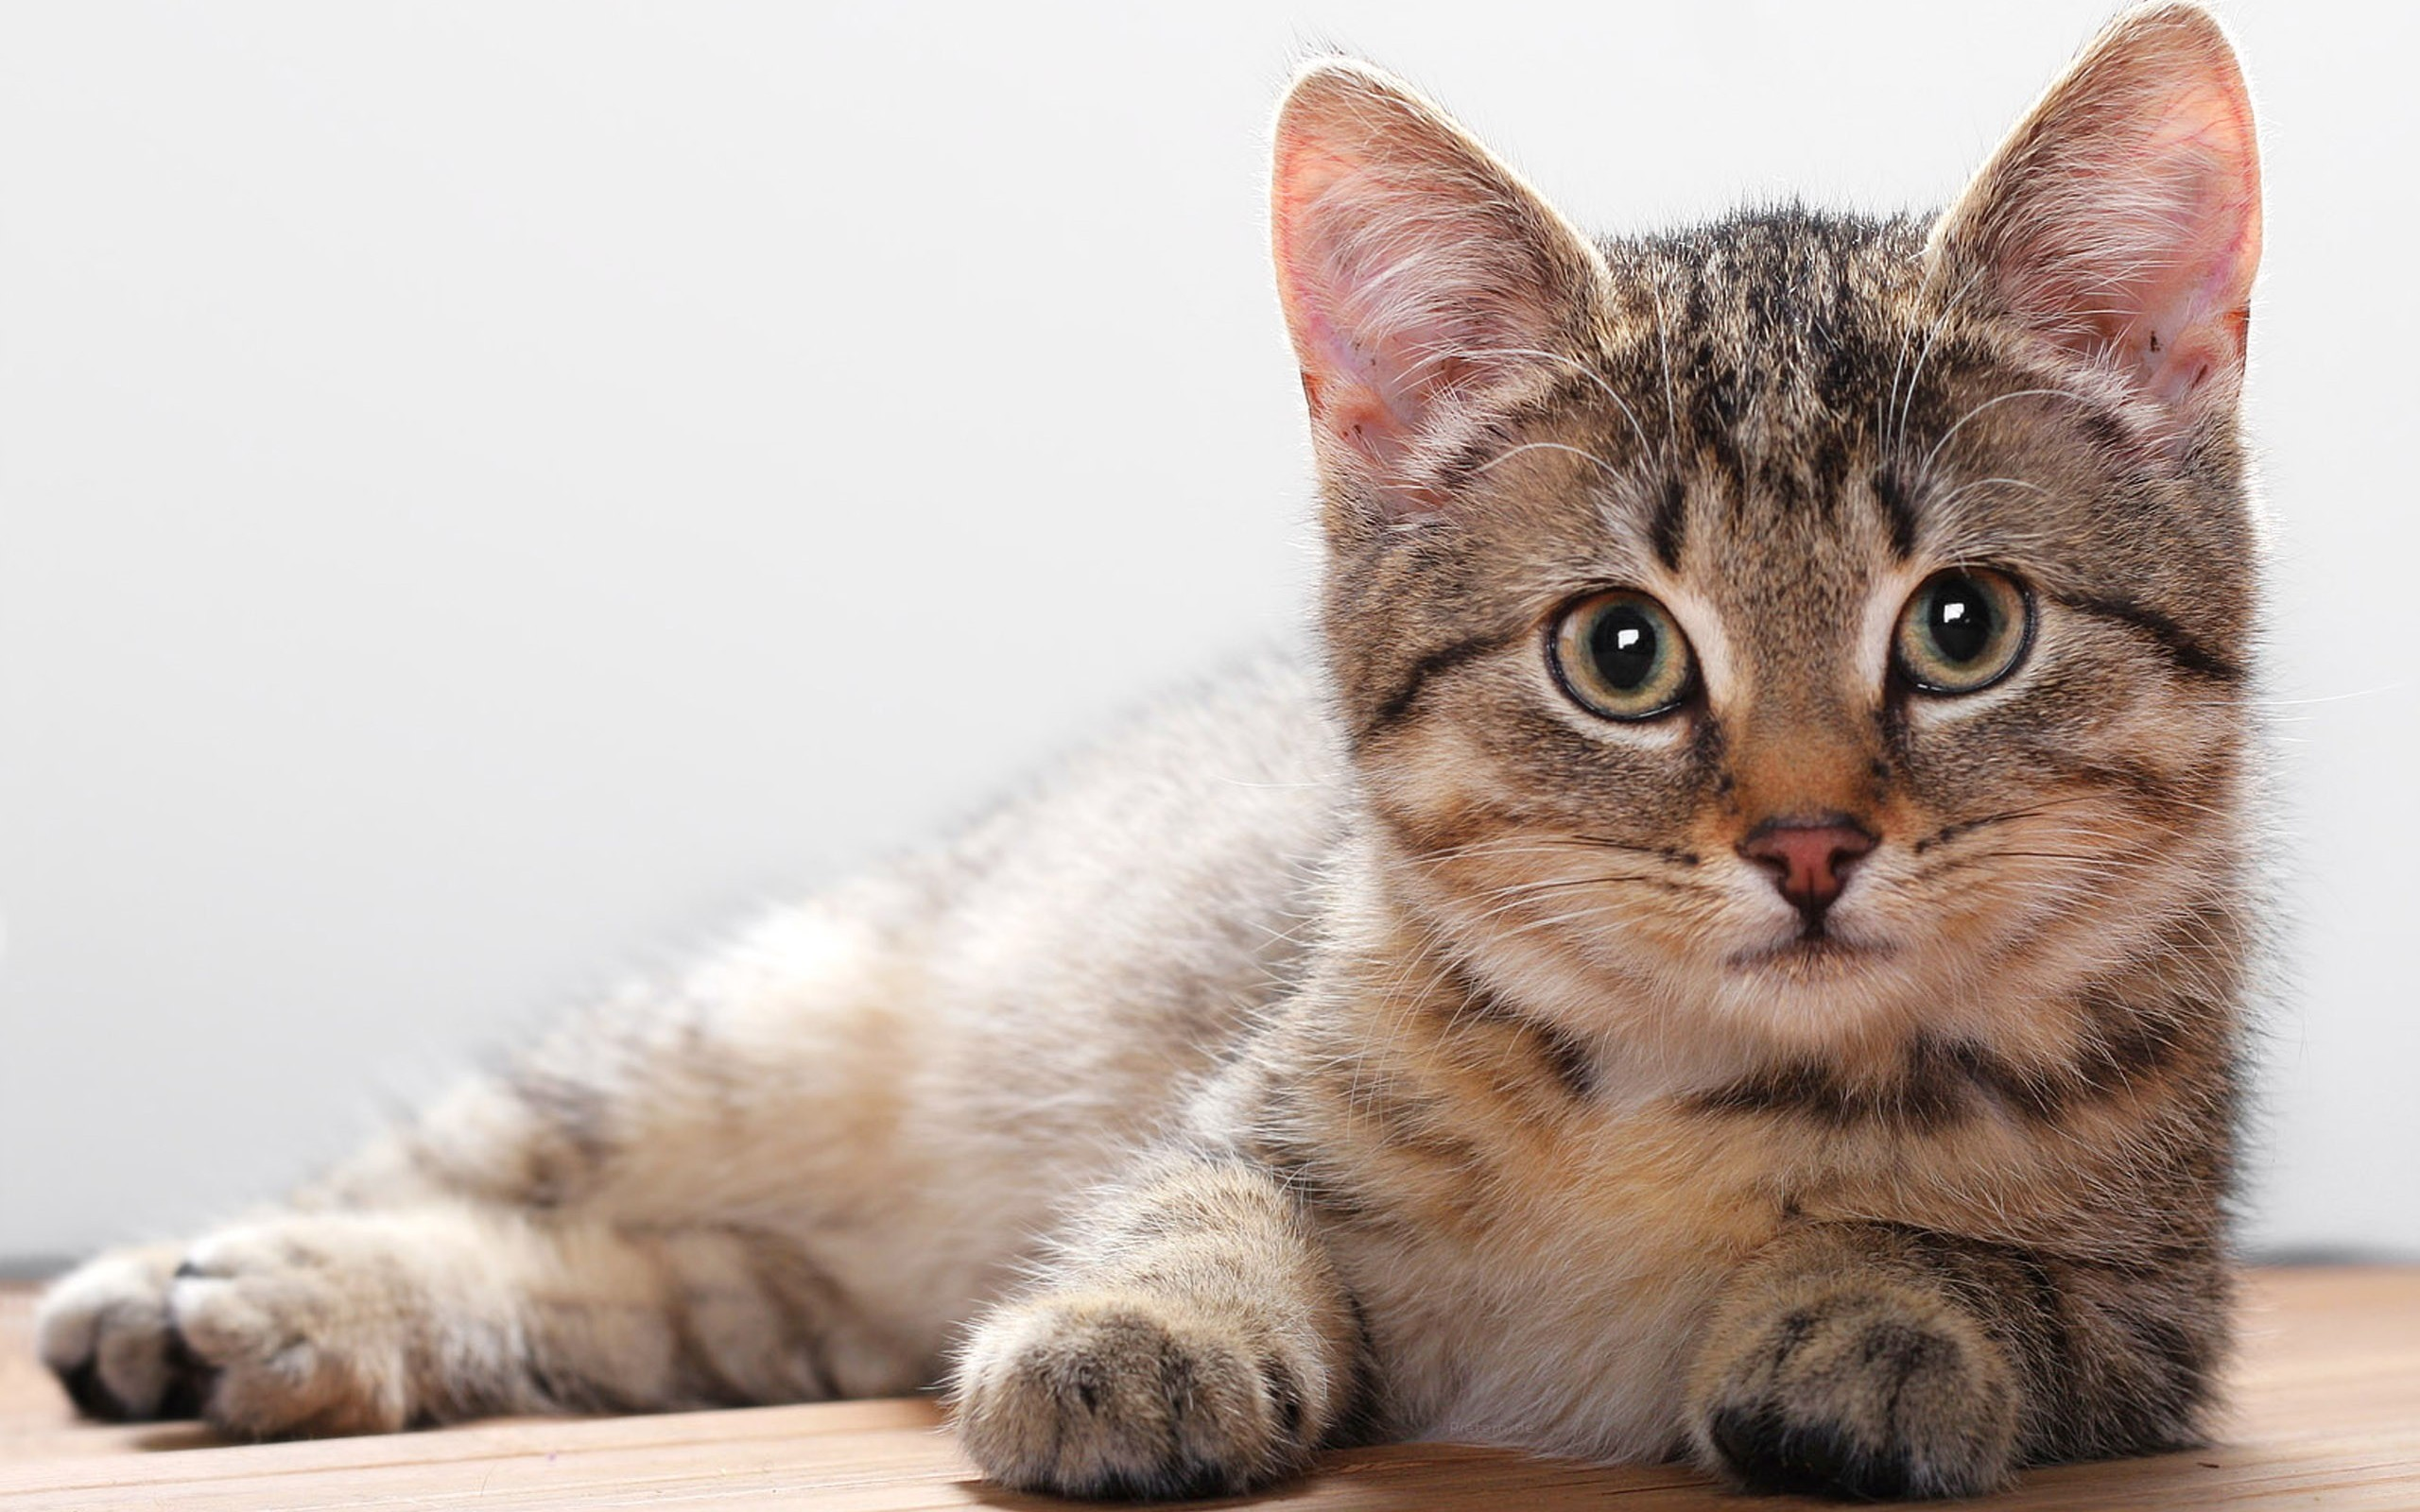
\includegraphics[scale=0.15]{cat}

    This is a cat $\varheart$
  }
  \only<2>{
    
\includegraphics[scale=0.2]{cat2}

    Still a cat $\varheart\varheart$
  }
  \only<3>{
    
\includegraphics[scale=0.3]{cat4}

    Half cat / half salad $\varheart\varheart\varheart$
  }
  \only<4>{
    
\includegraphics[scale=0.3]{cat3}

    Minecraft cat $\varheart\varheart\varheart\varheart$
  }
\end{slide}

% If the network learns to recgonize a feature in one layer
% Maybe it's good to keep that information for somewehere else too

\begin{slide}{Convolutional Neural Networks}
  \begin{itemize}
    \item Our network learns to detect a feature in one part of the image
    \pitem Wouldn't it make sense to reuse that information?
    % If the network learns to recognize a horizontal edge in the top left corner, then we want it to reuse that information elsewhere
    % Otherwise the neurons of each layer would need to re-learn that information
    \pitem Yes!
  \end{itemize}
  \vspace{0.5cm}
  {
    \Large
    Weight Sharing
  }
\end{slide}

\begin{slide}{Convolutional Neural Network: Mechanics}
  \frameheader{Recipe for a Convolutional Neural Network}
  \begin{itemize}
    \item<2-> Ingredients
    \begin{enumerate}
      \item<3-> Image $I$ with dimension $w \times h \times d$
      \item<4-> A kernel (filter) $K$ of size $k \times k \times d$
    \end{enumerate}
    \item<5-> Cooking
    \begin{itemize}
      \item<6-> \only<6>{Put the image into the oven at 150\degree C}\only<7->{Don't put the image into the oven at 150\degree C}
      \item<8-> Slide the kernel across the image
      \item<9-> Compute the ``dot product'' for each configuration
      \item<10-> (This is a convolution $I \ast K$)
    \end{itemize}
  \end{itemize}
\end{slide}

% \begin{slide}{Digression: Convolutions}
%   \begin{itemize}
%     \item<1-> Convolution is a mathematical operation
%     \item<2-> Used a lot in signal processing
%   \end{itemize}
%
%   \onslide<3->{
%     \begin{tikzpicture}
%       % x axis
%       \draw [->] (0, 0) -- (8.5, 0) node [below left] {$t$};
%
%       % y axis
%       \draw [->] (0, 0) -- (0, 2.5) node [below left] {$s(t)$};
%
%       % x Ticks
%       \foreach \i in {0, 1, ..., 7} {
%         \draw ({\i+0.5}, -0.1) node [below] {$\i$} -- ({\i+0.5}, 0);
%       }
%
%       % y Ticks
%       \foreach \i in {0, 1} {
%         \draw (-0.1, {\i+0.5}) node [left] {$\i$} -- (+0.1, {\i+0.5});
%       }
%
%       % Signal
%       \foreach \x in {0.5, 1, ..., 8} {
%         \draw [ProcessBlue] (\x, 0) -- (\x, {((rand+1)/2)*1.5});
%       }
%     \end{tikzpicture}
%   }
%   \onslide<4->{
%   \begin{tikzpicture}
%     % x axis
%     \draw [->] (0, 0) -- (2.3, 0) node [below left] {$t$};
%
%     % y axis
%     \draw [->] (0, 0) -- (0, 2.5) node [below left] {$k(t)$};
%
%     % x Ticks
%     \foreach \i in {0, 1, ..., 1.5} {
%       \draw ({\i+0.5}, -0.1) node [below] {$\i$} -- ({\i+0.5}, 0);
%     }
%
%     % y Ticks
%     \foreach \i in {0, 1} {
%       \draw (-0.1, {\i+0.5}) node [left] {$\i$} -- (+0.1, {\i+0.5});
%     }
%
%     % Signal
%     \foreach \x in {0.5, 1, ..., 1.5} {
%       \draw [Red] (\x, 0) -- (\x, {2-\x});
%     }
%   \end{tikzpicture}
%   }
% \end{slide}

\begin{slide}{Convolutional Neural Network: Mechanics}
  \begin{tikzpicture}
    % Image
    \draw (0, 0) grid ++(3, 3);

    % Grayscale pixel values
    \only<1>{
      \foreach \x in {0, ..., 2} {
        \foreach \y in {0, ..., 2} {
          \randomgray
          \fill [randomgray] (\x, \y) rectangle ++(1, 1);
        }
      }
    }

    \only<2-3>{
    \draw (0.5, 0.5) node {$0.8$};
    \draw (1.5, 0.5) node {$0.3$};
    \draw (2.5, 0.5) node {$0.5$};
    \draw (0.5, 1.5) node {$0.7$};
    \draw (1.5, 1.5) node {$0.2$};
    \draw (2.5, 1.5) node {$0.6$};
    \draw (0.5, 2.5) node {$0.4$};
    \draw (1.5, 2.5) node {$0.9$};
    \draw (2.5, 2.5) node {$0.1$};
    }

    \draw (1.5, -0.5) node {Image};

    \only<3-3>{
    \draw (4, 0) grid ++(2, 2);

    \draw (4.5, 0.5) node {$3.1$};
    \draw (5.5, 0.5) node {$0.9$};
    \draw (4.5, 1.5) node {$5.7$};
    \draw (5.5, 1.5) node {$2.4$};

    \draw (5, -0.5) node {Kernel};
    }

    \only<4-5>{
      \draw (0.5, 0.5) node {$0.8$};
      \draw (1.5, 0.5) node {$0.3$};
      \draw (2.5, 0.5) node {$0.5$};
      \draw (0.5, 1.5) node {\tiny$3.1 \cdot 0.7$};
      \draw (1.5, 1.5) node {\tiny$0.9 \cdot 0.2$};
      \draw (2.5, 1.5) node {$0.6$};
      \draw (0.5, 2.5) node {\tiny$5.7 \cdot 0.4$};
      \draw (1.5, 2.5) node {\tiny$2.4 \cdot 0.9$};
      \draw (2.5, 2.5) node {$0.1$};

      \draw [red] (0, 1) grid (2, 3);
    }
    \only<5-> {
      \draw [red] (4, 1) rectangle ++(1, 1) node [midway, black] {$6.79$};
      \draw (5, -0.5) node {Output};
    }
    \only<6-7>{
    \draw (0.5, 0.5) node {$0.8$};
    \draw (1.5, 0.5) node {$0.3$};
    \draw (2.5, 0.5) node {$0.5$};
    \draw (0.5, 1.5) node {$0.7$};
    \draw (1.5, 1.5) node {\tiny$3.1 \cdot 0.2$};
    \draw (2.5, 1.5) node {\tiny$0.9 \cdot 0.6$};
    \draw (0.5, 2.5) node {$0.4$};
    \draw (1.5, 2.5) node {\tiny$5.7 \cdot 0.9$};
    \draw (2.5, 2.5) node {\tiny$2.4 \cdot 0.1$};

      \draw [ProcessBlue] (1, 1) grid (3, 3);
    }
    \only<7-> {
      \draw [ProcessBlue] (5, 1) rectangle ++(1, 1) node [black, midway] {$6.53$};
    }
    \only<8-9>{
    \draw (0.5, 0.5) node {\tiny$3.1 \cdot 0.8$};
    \draw (1.5, 0.5) node {\tiny$0.9 \cdot 0.3$};
    \draw (2.5, 0.5) node {$0.5$};
    \draw (0.5, 1.5) node {\tiny$5.7 \cdot 0.7$};
    \draw (1.5, 1.5) node {\tiny$2.4 \cdot 0.2$};
    \draw (2.5, 1.5) node {$0.6$};
    \draw (0.5, 2.5) node {$0.4$};
    \draw (1.5, 2.5) node {$0.9$};
    \draw (2.5, 2.5) node {$0.1$};

      \draw [LimeGreen] (0, 0) grid (2, 2);
    }
    \only<9-> {
      \draw [LimeGreen] (4, 0) rectangle ++(1, 1) node [black, midway] {$7.67$};
    }
    \only<10-11>{
    \draw (0.5, 0.5) node {$0.8$};
    \draw (1.5, 0.5) node {\tiny$3.1 \cdot 0.3$};
    \draw (2.5, 0.5) node {\tiny$0.9 \cdot 0.5$};
    \draw (0.5, 1.5) node {$0.7$};
    \draw (1.5, 1.5) node {\tiny$5.7 \cdot 0.2$};
    \draw (2.5, 1.5) node {\tiny$2.4 \cdot 0.6$};
    \draw (0.5, 2.5) node {$0.4$};
    \draw (1.5, 2.5) node {$0.9$};
    \draw (2.5, 2.5) node {$0.1$};

      \draw [Magenta] (1, 0) grid (3, 2);
    }
    \only<11-> {
      \draw [Magenta] (5, 0) rectangle ++(1, 1) node [black, midway] {$3.96$};
    }
  \end{tikzpicture}
\end{slide}

\begin{slide}{Convolutional Neural Networks: Mechanics}
  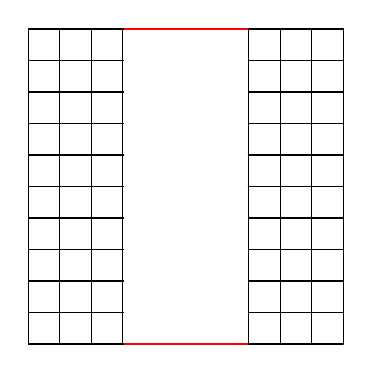
\begin{tikzpicture}
    % R layer (feature map)
    \yzplane{0}{
      \draw [ProcessBlue] (0, 0) rectangle ++(4, 4);
    }
    \xyplane{4}{
      \draw [ProcessBlue] (0, 0) rectangle ++(0.4, 4);
    }
    \xzplane{0}{
      \draw [ProcessBlue] (0, 0) rectangle ++(0.4, 4);
    }
    \xzplane{4}{
      \draw [ProcessBlue] (0, 0) rectangle ++(0.4, 4);
    }

    % G layer (feature map)
    \yzplane{0.4}{
      \draw [Green] (0, 0) rectangle ++(4, 4);
    }
    \xyplane{0}{
      \draw [Green] (0.4, 0) rectangle ++(0.4, 4);
    }
    \xyplane{4}{
      \draw [Green] (0.4, 0) rectangle ++(0.4, 4);
    }
    \xzplane{0}{
      \draw [Green] (0.4, 0) rectangle ++(0.4, 4);
    }
    \xzplane{4}{
      \draw [Green] (0.4, 0) rectangle ++(0.4, 4);
    }

    % B layer (feature map)
    \yzplane{0.8}{
      \draw [Red] (0, 0) rectangle ++(4, 4);
    }
    \xyplane{0}{
      \draw [Red] (0.8, 0) rectangle ++(0.4, 4);
    }
    \xyplane{4}{
      \draw [Red] (0.8, 0) rectangle ++(0.4, 4);
    }
    \xzplane{0}{
      \draw [Red] (0.8, 0) rectangle ++(0.4, 4);
    }
    \xzplane{4}{
      \draw [Red] (0.8, 0) rectangle ++(0.4, 4);
    }

    \foreach \i/\j in {0/1, 0.4/2, 0.8/3, 1.2/4, 1.6/5, 2.0/6, 2.4/7, 2.8/8} {
    \only<\j>{
      \xyplane{\i}{
        \draw (0, 2.79) grid [step=0.4] ++(1.2, 1.21);
      }
      \xyplane{{\i+1.2}}{
        \draw (0, 2.79) grid [step=0.4] ++(1.2, 1.21);
      }
      \yzplane{0}{
        \draw (2.79, \i) grid [step=0.4] ++(1.21, 1.21);
      }
      \yzplane{1.2}{
        \draw (2.79, \i) grid [step=0.4] ++(1.21, 1.21);
      }
      \xzplane{4}{
        \draw (0, \i) grid [step=0.4] ++(1.21, 1.21);
      }
      \xzplane{2.8}{
        \draw (0, \i) grid [step=0.4] ++(1.21, 1.21);
      }
    }
    }
  \end{tikzpicture}
\end{slide}

\begin{slide}{Convolutional Neural Network: Mechanics}
  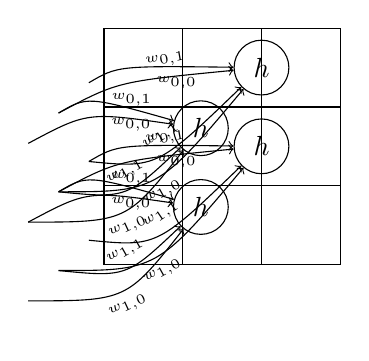
\begin{tikzpicture}
    \yzplane{0}{
      \foreach \y in {0, ..., 2} {
        \foreach \z in {0, ..., 2} {
          % \randomcolor
          % \fill [randomcolor] (\y, \z) rectangle ++(1, 1);
          \draw (\y, \z) rectangle ++(1, 1);
        }
      }
    }

    \newcount\slidecount\relax
    \slidecount=2\relax
    \foreach \i in {0, 1} {
      \foreach \j in {0, 1} {
        \only<\the\slidecount> {
          \path (2, {2.5-\i}, {2-\j*2})
                coordinate [draw, circle, inner sep=7pt]
                (h\j\i) node {$h$};

          \draw [->] (0, {2.5-\i}, {2.5-\j})
             .. controls (0.75, {2.9-\i}, {2.5-\j}) .. (h\j\i)
             node [pos=0.6, above right, sloped] {\tiny$w_{0,1}$};

          \draw [->] (0, {2.5-\i}, {1.5-\j})
             .. controls (0.75, {3.1-\i}, {2.5-\j}) .. (h\j\i)
             node [pos=0.8, below] {\tiny$w_{0,0}$};

          \draw [->] (0, {1.5-\i}, {2.5-\j})
            .. controls (1.25, {1.5-\i}, {2.5-\j}) .. (h\j\i)
             node [pos=0.5, below, sloped] {\tiny$w_{1,0}$};

          \draw [->] (0, {1.5-\i}, {1.5-\j})
            .. controls (1.25, {1.8-\i}, {2.5-\j}) .. (h\j\i)
             node [pos=0.6, above, sloped] {\tiny$w_{1,1}$};
        }
        \global\advance\slidecount by 1\relax
      }
    }

  \end{tikzpicture}
  % Most importantly, we'd most often have many kernels for each layer
  % So if the input layer has k feature maps, the output layer will have x feature maps
\end{slide}

\begin{slide}{Convolutional Neural Network: Hyperparameters}
  \begin{itemize}
    \item<1-> Convolutional Neural Networks have three hyperparameters
    \begin{enumerate}
      \item<2-> Kernel size % usually odd for valid padding, 3x3 or 5x5
      \item<3-> Kernel stride % usually 1 or 2
      \item<4-> Padding (valid or same)
      % Valid we don't go past th edge, so the spatial dimension will reduce
      % Same padding we do go past the edge and pad the image with zeros
      % then the spatial dimension will stay the same (most common)
    \end{enumerate}
  \end{itemize}
  \vspace{1cm}

  \onslide<4->{
    \begin{tikzpicture}
      \draw (0, 0) grid [step=0.5] (2, 2);
      \foreach \i/\s in {0/5, 0.5/6} {
        \only<\s>{
          \fill [red] (\i, 0.5) rectangle ++(1.5, 1.5);
          \draw (\i, 0.5) grid [step=0.5] ++(1.5, 1.5);
        }
      }
      \newcommand{\drawzeros}{
        \foreach \i in {0, 0.5, ..., 1.5} {
          \draw (\i, -0.5) rectangle ++(0.5, 0.5) node [midway] {0};
          \draw (-0.5, \i) rectangle ++(0.5, 0.5) node [midway] {0};
          \draw (\i, 2) rectangle ++(0.5, 0.5) node [midway] {0};
          \draw (2, \i) rectangle ++(0.5, 0.5) node [midway] {0};
        }
        \foreach \i in {-0.5, 2} {
          \draw (\i, -0.5) rectangle ++(0.5, 0.5) node [midway] {0};
          \draw (\i, 2) rectangle ++(0.5, 0.5) node [midway] {0};
        }
      }
      \only<7-> {
        \drawzeros
      }
      \foreach \i/\s in {-0.5/8, 0/9, 0.5/10, 1/11} {
        \only<\s>{
          \fill [red] (\i, 1) rectangle ++(1.5, 1.5);
          \draw ({\i+0.5}, 1.5) rectangle ++(0.5, 0.5) node [midway] {$\times$};
          \draw (\i, 1) grid [step=0.5] ++(1.5, 1.5);
          \drawzeros
        }
      }
    \end{tikzpicture}
  }
\end{slide}

\begin{frame}[fragile]{Convolutional Neural Networks: Pooling}
  \begin{itemize}
    \item<1-> \emph{Pooling} achieves translational invariance
    \item<2-> A form of downsampling
    \item<3-> The maximum stays the maximum
    % Pooling reduces the width and height, convolutions modify the depth
  \end{itemize}
  \vspace{0.5cm}

  \begin{center}
  \begin{tikzpicture}
    \newcommand{\numbergrid}[4]{%
      \draw (0, 0) rectangle ++(1, 1) node [midway] {#1};%
      \draw (1, 0) rectangle ++(1, 1) node [midway] {#2};%
      \draw (0, 1) rectangle ++(1, 1) node [midway] {#3};%
      \draw (1, 1) rectangle ++(1, 1) node [midway] {#4};%
    }
    \only<3> {\numbergrid{6}{32}{66}{2}}
    \only<4> {\numbergrid{66}{32}{6}{2}}
    \only<5> {\numbergrid{6}{32}{2}{66}}
    \only<6> {\numbergrid{2}{66}{32}{6}}
  \end{tikzpicture}
\end{center}
\end{frame}

\begin{slide}{Convolutional Neural Network: Architecture}
  \texttt{INPUT ->}

  \texttt{[[CONV -> RELU]*N -> POOL?]*M ->}

  \texttt{[FC -> RELU]*K -> FC}

  \begin{flushleft}\cite{karpathy1}\end{flushleft}
\end{slide}

\begin{slide}{Convolutional Neural Networks: Intuition}
  \begin{itemize}
    \pitem Each layer of a ConvNet learns to detect features
    \pitem Later layers combine features of earlier layers
    \pitem For early layers, we can still gain an intuition of what they do
  \end{itemize}
\end{slide}

\begin{slide}{Convolutional Neural Networks: Intuition}
  \frameheader{What's in a kernel?}

  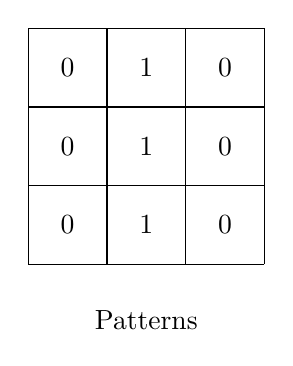
\begin{tikzpicture}
    \draw (0, 0) grid ++(3, 3);
    \foreach \i in {0, ..., 2} {
      \foreach \j in {0, ..., 2} {
        \ifnum\i=1
          \draw ({\i+0.5}, {\j+0.5}) node {1};
        \else
          \draw ({\i+0.5}, {\j+0.5}) node {0};
        \fi
      }
    }

      \draw (1.5, -0.7) node {Patterns};
      % 1. patterns
      % other things
  \end{tikzpicture}
\end{slide}

\begin{slide}{Convolutional Neural Networks: Intuition}
  \frameheader{What's in a kernel?}

  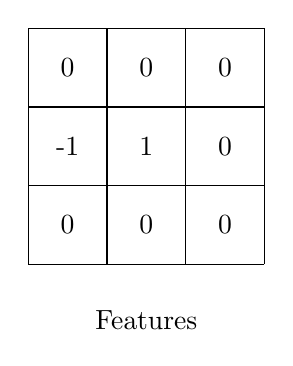
\begin{tikzpicture}
    \draw (0, 0) grid ++(3, 3);
    \foreach \i in {0, ..., 2} {
      \foreach \j in {0, ..., 2} {
        \ifnum\j=1
          \ifnum\i=0
            \draw ({\i+0.5}, {\j+0.5}) node {-1};
          \else
            \ifnum\i=1
              \draw ({\i+0.5}, {\j+0.5}) node {1};
            \else
              \draw ({\i+0.5}, {\j+0.5}) node {0};
            \fi
          \fi
        \else
          \draw ({\i+0.5}, {\j+0.5}) node {0};
        \fi
      }
    }

      % When the two pixels are similar, the two values cancel
      % When they are different (near edges), they give a large value
      \draw (1.5, -0.7) node {Features};
      % 1. patterns
      % other things
  \end{tikzpicture}
\end{slide}

\begin{slide}{Convolutional Neural Networks: Intuition}
  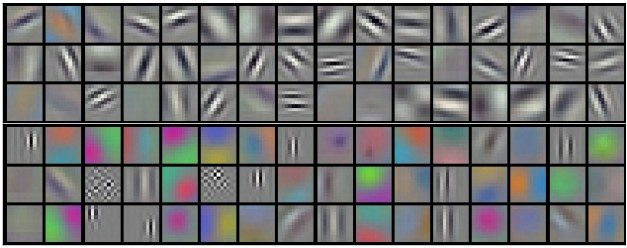
\includegraphics[scale=0.45]{weights}
\end{slide}

\begin{slide}{Case Study: AlexNet}
  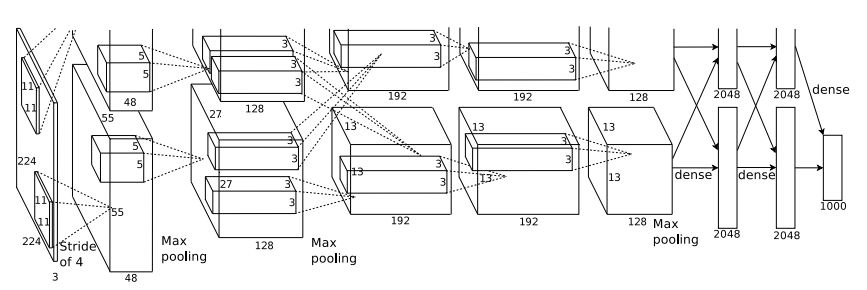
\includegraphics[scale=0.45]{alexnet}
\end{slide}

% RNNs and LSTM

\begin{slide}{Sequences}
  \begin{itemize}
    \item<2-> Humans think in sequences
    \item<3-> Sequences give single entities context
    \item<5-> The key to understanding sequences is memory
  \end{itemize}
  \vspace{0.5cm}

  \onslide<3->{I }\onslide<4->{enjoy }\onslide<3->{eat}\onslide<4->{ing dinner with }\onslide<3->{people}
\end{slide}

\begin{slide}{Machine Memory}
  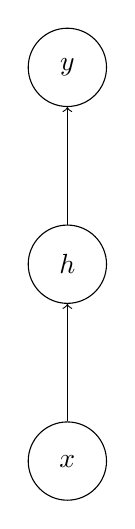
\begin{tikzpicture}
    % Nodes
    \path (0, 0) coordinate [draw, circle, inner sep=10pt] (x) node {$x$};
    \path (0, 2.5) coordinate [draw, circle, inner sep=10pt] (h) node {$h$};
    \path (0, 5) coordinate [draw, circle, inner sep=10pt] (y) node {$y$};

    % Connections
    \draw [->] (x) -- (h);
    \draw [->] (h) -- (y);
  \end{tikzpicture}
\end{slide}

\begin{frame}[fragile]{Machine Memory}
  \begin{center}
  \begin{tikzpicture}
    % Nodes
    \path (0, 0) coordinate [draw, circle, inner sep=10pt] (x) node {$x_t$};
    \path (0, 2.5) coordinate [draw, circle, inner sep=10pt] (h) node {$h_t$};
    \path (0, 5) coordinate [draw, circle, inner sep=10pt] (y) node {$y_t$};

    % Connections
    \draw [->] (x) -- (h);
    \draw [->] (h) -- (y);

    \newcommand{\timestep}[2]{
      % Nodes
      \path (#1, 0) coordinate [draw, circle, inner sep=10pt]
            (x#2) node {$x_{t+#2}$};
      \path (#1, 2.5) coordinate [draw, circle, inner sep=10pt]
            (h#2) node {$h_{t+#2}$};
      \path (#1, 5) coordinate [draw, circle, inner sep=10pt]
            (y#2) node {$y_{t+#2}$};

      % Connections
      \draw [->] (x#2) -- (h#2);
      \draw [->] (h#2) -- (y#2);
    }

    \only<2> {
      \draw [->] (h) [out=45,in=-45,looseness=5] to (h);
      \draw (1.6, 2.5) node {$h_{t-1}$};
    }

    \only<3-> {
      \timestep{2}{1}
      \draw [->] (h) -- (h1);
    }
    \only<4-> {
      \timestep{4}{2}
      \draw [->] (h1) -- (h2);
    }
    \only<5-> {
      \timestep{6}{3}
      \draw [->] (h2) -- (h3);
    }
    \only<6-> {
      \timestep{8}{4}
      \draw [->] (h3) -- (h4);
    }
  \end{tikzpicture}
  \end{center}
\end{frame}

\begin{slide}{Machine Memory}
  $$h_t = f(w \cdot x + b)$$
\end{slide}

\begin{slide}{Machine Memory}
  $$h_t = f(\mathbf{w}^\top [h_{t-1}, x] + b)$$
\end{slide}

\begin{slide}{Recurrent Neural Networks}
  \begin{itemize}
    \pitem Recurrent Neural Networks (RNNs) share weights through time
    \pitem They have \emph{memory}
    \pitem And they have a problem:
  \end{itemize}
  \vspace{1cm}
  {
    \Large
    The Vanishing Gradient Problem
  }
\end{slide}

% \begin{frame}[fragile]{Machine Memory}
%   \begin{center}
%   \begin{tikzpicture}
%     % Nodes
%     \path (0, 0) coordinate [draw, circle, inner sep=10pt] (x) node {$x_t$};
%     \path (0, 2.5) coordinate [draw, circle, inner sep=10pt] (h) node {$h_t$};
%     \path (0, 5) coordinate [draw, circle, inner sep=10pt] (y) node {$y_t$};
%
%     % Connections
%     \only<1>{\draw [->] (x) -- (h);}
%     \only<2>{\draw [->] (x) -- (h) node [left, midway] {$w$};}
%     \draw [->] (h) -- (y);
%
%     \newcommand{\timestep}[2]{
%       % Nodes
%       \path (#1, 0) coordinate [draw, circle, inner sep=10pt]
%             (x#2) node {$x_{t+#2}$};
%       \path (#1, 2.5) coordinate [draw, circle, inner sep=10pt]
%             (h#2) node {$h_{t+#2}$};
%       \path (#1, 5) coordinate [draw, circle, inner sep=10pt]
%             (y#2) node {$y_{t+#2}$};
%
%       % Connections
%       \only<1>{\draw [->] (x#2) -- (h#2);}
%       \only<2->{\draw [->] (x#2) -- (h#2) node [left, midway] {$w$};}
%       \draw [->] (h#2) -- (y#2);
%     }
%
%     \timestep{2}{1}
%     \draw [->] (h) -- (h1);
%
%     \timestep{4}{2}
%     \draw [->] (h1) -- (h2);
%   \end{tikzpicture}
%   \end{center}
% \end{frame}
%
% \begin{frame}[fragile]{Machine Memory}
%   \begin{center}
%   \begin{tikzpicture}
%     % Nodes
%     \path (0, 0) coordinate [draw, circle, inner sep=10pt] (x) node {$x_t$};
%     \path (0, 2.5) coordinate [draw, circle, inner sep=10pt] (h) node {$h_t$};
%     \path (0, 5) coordinate [draw, circle, inner sep=10pt] (y) node {$y_t$};
%     \path (0, 1.25) coordinate [draw, circle, inner sep=7pt]
%           (w) node {$w$};
%
%     % Connections
%     \draw [->] (x) -- (w);
%     \draw [->] (w) -- (h);
%     \draw [->] (h) -- (y);
%
%     \newcommand{\timestep}[2]{
%       % Nodes
%       \path (#1, 0) coordinate [draw, circle, inner sep=10pt]
%             (x#2) node {$x_{t+#2}$};
%       \path (#1, 2.5) coordinate [draw, circle, inner sep=10pt]
%             (h#2) node {$h_{t+#2}$};
%       \path (#1, 5) coordinate [draw, circle, inner sep=10pt]
%             (y#2) node {$y_{t+#2}$};
%       \path (#1, 1.25) coordinate [draw, circle, inner sep=7pt]
%             (w#2) node {$w$};
%
%       % Connections
%       \draw [->] (x#2) -- (w#2);
%       \draw [->] (w#2) -- (h#2);
%       \draw [->] (h#2) -- (y#2);
%     }
%
%     \timestep{2}{1}
%     \draw [->] (h) -- (h1);
%
%     \timestep{4}{2}
%     \draw [->] (h1) -- (h2);
%   \end{tikzpicture}
%   \end{center}
% \end{frame}
%
% \begin{frame}[fragile]{Machine Memory}
%   \begin{center}
%   \begin{tikzpicture}
%     % Nodes
%     \path (0, 0) coordinate [draw, circle, inner sep=10pt] (x) node {$x_t$};
%     \path (0, 2.5) coordinate [draw, circle, inner sep=10pt] (h) node {$h_t$};
%     \path (0, 5) coordinate [draw, circle, inner sep=10pt] (y) node {$y_t$};
%     \path (0, 1.25) coordinate [draw, circle, inner sep=7pt]
%           (w) node {$w$};
%
%     % Connections
%     \draw [->] (x) -- (w);
%     \draw [->] (w) -- (h);
%     \draw [->] (h) -- (y);
%
%     \newcommand{\timestep}[2]{
%       % Nodes
%       \path (#1, 0) coordinate [draw, circle, inner sep=10pt]
%             (x#2) node {$x_{t-#2}$};
%       \path (#1, 2.5) coordinate [draw, circle, inner sep=10pt]
%             (h#2) node {$h_{t-#2}$};
%       \path (#1, 5) coordinate [draw, circle, inner sep=10pt]
%             (y#2) node {$y_{t-#2}$};
%       \path (#1, 1.25) coordinate [draw, circle, inner sep=7pt]
%             (w#2) node {$w$};
%
%       % Connections
%       \draw [->] (x#2) -- (w#2);
%       \draw [->] (w#2) -- (h#2);
%       \draw [->] (h#2) -- (y#2);
%     }
%
%     \timestep{-2}{1}
%     \draw [->] (h) -- (h1);
%
%     \timestep{-4}{2}
%     \draw [->] (h1) -- (h2);
%   \end{tikzpicture}
%   \end{center}
% \end{frame}
%
% \begin{frame}[fragile]{Machine Memory}
%   \begin{center}
%   \begin{tikzpicture}
%     % Nodes
%     \path (0, 2.5) coordinate [draw, circle, inner sep=10pt] (h) node {$h_t$};
%     \path (0, 5) coordinate [draw, circle, inner sep=10pt] (y) node {$y_t$};
%     \path (0, 1.25) coordinate [draw, circle, inner sep=7pt]
%           (w) node {$w$};
%
%     % Connections
%     \draw [->] (w) -- (h);
%     \draw [->] (h) -- (y);
%
%     \newcommand{\timestep}[2]{
%       % Nodes
%       \path (#1, 2.5) coordinate [draw, circle, inner sep=10pt]
%             (h#2) node {$h_{t-#2}$};
%       \path (#1, 1.25) coordinate [draw, circle, inner sep=7pt]
%             (w#2) node {$w$};
%
%       % Connections
%       \draw [->] (w#2) -- (h#2);
%     }
%
%     \timestep{-2}{1}
%     \draw [->] (h) -- (h1);
%
%     \timestep{-4}{2}
%     \draw [->] (h1) -- (h2);
%   \end{tikzpicture}
%   \end{center}
% \end{frame}
%
% \begin{frame}[fragile]{Machine Memory}
%   \begin{center}
%   \begin{tikzpicture}
%     % Weight
%     \path (-2, 0) coordinate [draw, circle, inner sep=7pt]
%           (w) node {$w$};
%
%     % Nodes
%     \path (0, 2.5) coordinate [draw, circle, inner sep=10pt] (h) node {$h_t$};
%     \path (0, 5) coordinate [draw, circle, inner sep=10pt] (y) node {$y_t$};
%
%     % Connections
%     \only<1>{\draw [->] (h) -- (y);}
%     \only<2->{
%       \draw [red, ->] (h) -- (y)
%             node [black, right, midway] {$\frac{\partial y_t}{\partial h_t}$};
%     }
%     \only<-2>{\draw [->] (w) -- (h);}
%     \only<3->{
%       \draw [red, ->] (w) -- (h)
%             node [black, right, pos=0.7] {$\frac{\partial h_t}{\partial w}$};
%     }
%
%     % Nodes
%     \path (-2, 2.5) coordinate [draw, circle, inner sep=10pt]
%           (h1) node {$h_{t-1}$};
%     % Connections
%     \only<-4>{\draw [->] (w) -- (h1);}
%     \only<5->{
%       \draw [red, ->] (w) -- (h1)
%             node [black, right, pos=0.7] {$\frac{\partial h_{t-1}}{\partial w}$};
%     }
%     \only<-3>{\draw [->] (h) -- (h1);}
%     \only<4->{
%       \draw [red, ->] (h) -- (h1)
%             node [black, above, midway] {$\frac{\partial h_t}{\partial h_{t-1}}$};
%     }
%
%     \path (-4, 2.5) coordinate [draw, circle, inner sep=10pt]
%           (h2) node {$h_{t-2}$};
%     % Connections
%     \only<-6>{\draw [->] (w) -- (h2);}
%     \only<7->{
%       \draw [red, ->] (w) -- (h2)
%             node [black, pos=0.7, right] {$\frac{\partial h_{t-2}}{\partial w}$};
%     }
%     \only<-5>{\draw [->] (h1) -- (h2);}
%     \only<6->{
%       \draw [red, ->] (h1) -- (h2)
%             node [black, above, midway] {$\frac{\partial h_{t-1}}{\partial h_{t-2}}$};
%     }
%
%     \only<7-> {
%     \path (-7, 2.5) coordinate [draw, circle, inner sep=10pt]
%           (1) node {$h_1$};
%       \draw [semithick, dotted, ->] (h2) -- (1);
%       \draw [->] (w) -- (1);
%     }
%     \onslide<8>{
%     \draw (-3, -1) node {%
%       $
%         \frac{\partial h_t}{\partial h_{t-1}}
%         \frac{\partial h_{t-1}}{\partial h_{t-2}}
%         \frac{\partial h_{t-2}}{\partial h_{t-3}}
%         \dotsm
%         \frac{\partial h_2}{\partial h_1}
%       $
%     };
%     }
%     \onslide<9>{
%       \draw (-3, -1) node {$0.1 \cdot 0.1 \cdot 0.1 \dotsm 0.1$};
%     }
%     \onslide<10>{
%       \draw (-3, -1) node {$0.1 \cdot 0.1 \cdot 0.1 \dotsm 0.1 \approx 0$};
%     }
%   \end{tikzpicture}
%   \end{center}
% \end{frame}

\begin{slide}{LSTMs}
  \begin{itemize}
    \item<1-> RNN's are forgetful
    \item<2-> \emph{Long Short Term Memory} (LSTM) Units solve this problem
    \item<3-> Developed by Schmidhuber and Hochreiter at TUM in 1997
  \end{itemize}
\end{slide}

% First explain what an LSTM consists of

\begin{slide}{LSTMs}
  \begin{itemize}
    \pitem LSTMs are a lot like flip-flops
    \pitem They have three \emph{gates}
    \begin{itemize}
      \pitem Input gate
      \pitem Forget gate
      \pitem Output gate
    \end{itemize}
  \end{itemize}
  \vspace{0.5cm}
  \pause
  $G_i(x_t, h_{t-1}) = \sigma(\mathbf{w}_i^\top [x_t, h_{t-1}] + b_i)$
\end{slide}

\begin{slide}{LSTMs}
  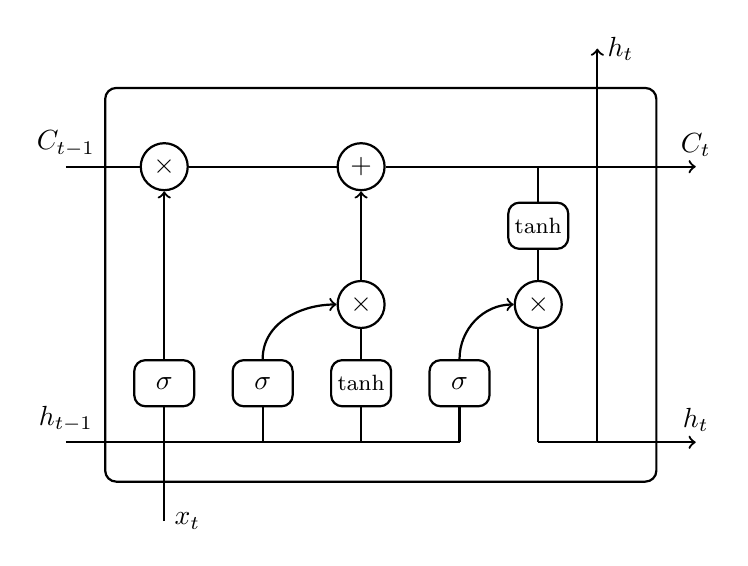
\begin{tikzpicture}[thick]
    % Unit
    \draw [rounded corners, thick] (0, 0) rectangle (7, 5);

    % Conveyor Belt
    \path (0.75, 4) coordinate [draw, circle, thick, inner sep=6pt]
          (m1) node {$\times$};
    \path (3.25, 4) coordinate [draw, circle, thick, inner sep=6pt]
          (add) node {$+$};
    \draw [thick, ->]
          (-0.5, 4) node [above] {$C_{t-1}$}
       -- (m1)
       -- (add)
       -- (7.5, 4) node [above] {$C_t$};

    % previous activation input
   \path (-0.5, 0.5) coordinate (hp) node [above] {$h_{t-1}$};

    % input
    \path (0.75, -0.5) coordinate (x) node [right] {$x_t$};

    % output
    \path (6.25, 5.5) coordinate (h1) node [right] {$h_t$};

    \path (7.5, 0.5) coordinate (h2) node [above] {$h_t$};

    % forget gate
    \path (0.75, 1.25) coordinate
          [draw, rectangle, rounded corners, thick, text width=15pt, text height=10pt]
          (fg);
    \draw (fg) node {$\sigma$};
    \coordinate (a1) at (0.75, 0.5);

    % input gate
    \path (2, 1.25) coordinate
          [draw, rectangle, rounded corners, thick, text width=15pt, text height=10pt]
          (ig);
    \draw (ig) node {$\sigma$};
    \coordinate (a2) at (2, 0.5);

    % Activation function
    \path (3.25, 1.25) coordinate
          [draw, rectangle, rounded corners, thick, text width=15pt, text height=10pt]
          (f1);
    \draw (f1) node {\footnotesize$\tanh$};
    \coordinate (a3) at (3.25, 0.5);

    \path (f1)+(0, 1) coordinate [draw, circle, thick, inner sep=6pt]
          (m2) node {$\times$};

    % output gate
    \path (4.5, 1.25) coordinate
          [draw, rectangle, rounded corners, thick, text width=15pt, text height=10pt]
          (og);
    \draw (og) node {$\sigma$};
    \coordinate (a4) at (4.5, 0.5);

    % Output activation
    \path (5.5, 3.25) coordinate
          [draw, rectangle, rounded corners, thick, text width=15pt, text height=10pt]
          (f2);
    \draw (f2) node {\footnotesize$\tanh$};
    \coordinate (a5) at (5.5, 4);
    \coordinate (a6) at (5.5, 0.5);
    \coordinate (a7) at (6.25, 0.5);

    \path (f2)+(0, -1) coordinate [draw, circle, thick, inner sep=6pt]
          (m3) node {$\times$};

    % Connections
    \draw (hp) -- (a1) -- (a2) -- (a3) -- (a4);
    \draw (x) -- (a1);

    % Forget gate
    \draw (a1) -- (fg);
    \draw [->] (fg) -- (m1);

    % Input gate
    \draw (a2) -- (ig);

    % Input activation
    \path [->] (ig) edge [out=90, in=180] (m2);
    \draw (a3) -- (f1);
    \draw (f1) -- (m2);
    \draw [->] (m2) -- (add);

    % Output gate
    \draw (a4) -- (og);
    \path [->] (og) edge [out=90, in=180] (m3);

    % Output activation
    \draw (a5) -- (f2);
    \draw (f2) -- (m3);
    \draw (m3) -- (a6);
    \draw (a6) -- (a7);
    \draw [->] (a7) -- (h1);
    \draw [->] (a7) -- (h2);

  \end{tikzpicture}
\end{slide}

\begin{slide}{LSTMs}
  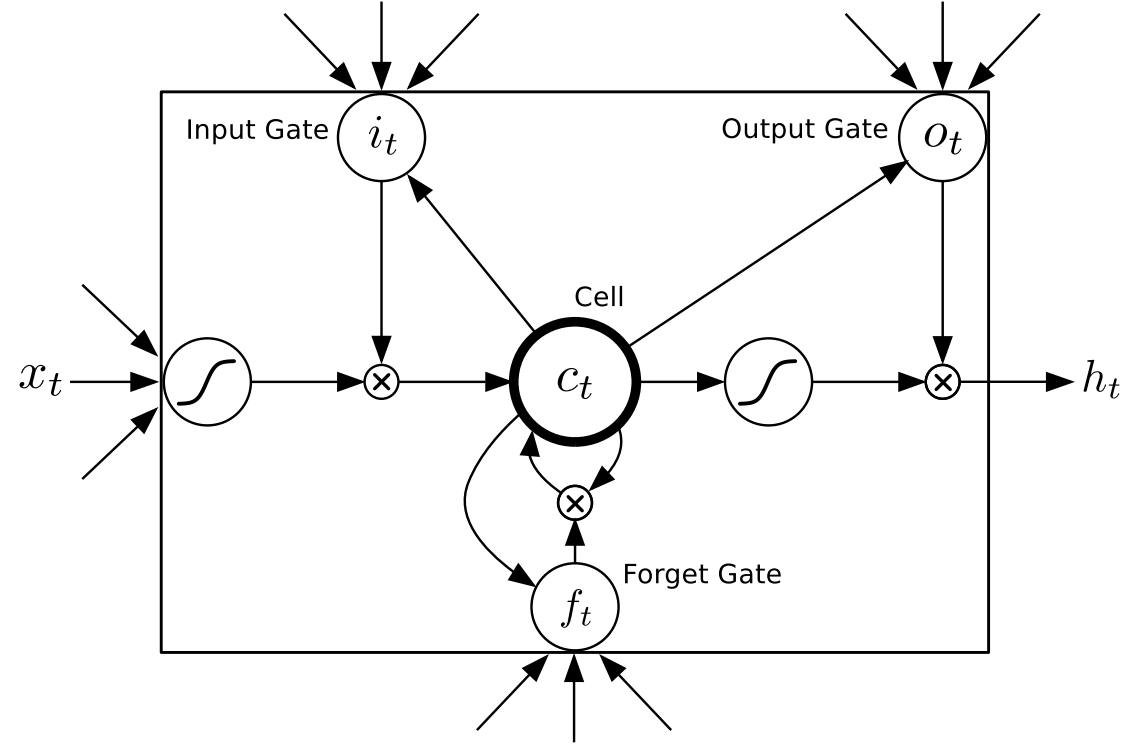
\includegraphics[scale=0.5]{lstm};
\end{slide}

\begin{slide}{LSTMs: What can they do?}
  \frameheader{So, what can LSTMs actually do?}
\end{slide}

\begin{slide}{LSTMs: What can they do?}
  % trained an LSTM of Leo Tolstoy’s War and Peace and then generated samples every 100 iterations of training
  % Understands that words are delimited by spaces
  \begin{quote}
    tyntd-iafhatawiaoihrdemot  lytdws  e ,tfti, astai f ogoh eoase rrranbyne 'nhthnee e plia tklrgd t o idoe ns,smtt   h ne etie h,hregtrs nigtike,aoaenns lng
  \end{quote}
  \vspace{0.25cm}
  Iteration: 100
\begin{flushleft}\cite{lstm}\end{flushleft}
\end{slide}

\begin{slide}{LSTMs: What can they do?}
  % quotes, peridos
  \begin{quote}
    ``Tmont thithey'' fomesscerliund
      Keushey. Thom here
      sheulke, anmerenith ol sivh I lalterthend Bleipile shuwy fil on aseterlome
      coaniogennc Phe lism thond hon at. MeiDimorotion in ther thize."
  \end{quote}
  \vspace{0.25cm}
  Iteration: 300
\begin{flushleft}\cite{lstm}\end{flushleft}
\end{slide}

\begin{slide}{LSTMs: What can they do?}
  % real words
  \begin{quote}
    we counter. He stutn co des. His stanted out one ofler that concossions and was to gearang reay Jotrets and with fre colt otf paitt thin wall. Which das stimn
  \end{quote}
  \vspace{0.25cm}
  Iteration: 500
\begin{flushleft}\cite{lstm}\end{flushleft}
\end{slide}

\begin{slide}{LSTMs: What can they do?}
  % more real words
  \begin{quote}
    Aftair fall unsuch that the hall for Prince Velzonski's that me of
    her hearly, and behs to so arwage fiving were to it beloge, pavu say falling misfort
    how, and Gogition is so overelical and ofter.
  \end{quote}
  \vspace{0.25cm}
  Iteration: 700
\begin{flushleft}\cite{lstm}\end{flushleft}
\end{slide}

\begin{slide}{LSTMs: What can they do?}
  % more real words
  \begin{quote}
    ``Why do what that day,'' replied Natasha, and wishing to himself the fact the princess, Princess Mary was easier, fed in had oftened him. Pierre aking his soul came to the packs and drove up his father-in-law women.
  \end{quote}
  \vspace{0.25cm}
  Iteration: 2000
\begin{flushleft}\cite{lstm}\end{flushleft}
\end{slide}

\begin{slide}{LSTMs: What can they do?}
  {
    \huge
    They can write Linux kernel code!
  }
\end{slide}

\begin{slide}{LSTMs: What can they do?}
  {
    \huge
    They can compose music!
  }
\end{slide}


\begin{slide}{Deep Learning}
  \begin{itemize}
    \pitem Why the recent success of deep learning? %Why did it take so long for deep learning to take off?
    \pitem Three reasons
    \begin{enumerate}
      \pitem Better hardware
      \pitem More data
      \pitem Better methods
    \end{enumerate}
  \end{itemize}
\end{slide}

\begin{slide}{Deep Learning}
  {
    \Huge
    The Ugly
  }
\end{slide}
